\section{Web Search Agent: Quality Evaluation with DeepEval}

This section presents an experimental validation of the Web Search Agent (Workflow 4), which integrates real-time information retrieval via Google Search, LLM-based summarization, and automated quality assessment using DeepEval metrics. The evaluation demonstrates the system's ability to provide reliable, fact-checked technical guidance for STM32 embedded AI development.

\subsection{Methodology}

\subsubsection{Evaluation Framework}
The quality assessment utilizes \textbf{DeepEval}\footnote{\url{https://github.com/confident-ai/deepeval}}, an open-source framework designed for RAG (Retrieval-Augmented Generation) evaluation. The framework was configured as follows:

\begin{itemize}
  \item \textbf{LLM Backend}: Mistral (7B parameters) via Ollama, running locally at \texttt{http://localhost:11434}
  \item \textbf{Metrics}: Four domain-specific metrics tailored for technical documentation:
        \begin{itemize}
          \item \textbf{Faithfulness}: Measures factual consistency between the LLM-generated summary and retrieved documents (range: 0.0--1.0, higher is better)
          \item \textbf{Answer Relevancy}: Assesses semantic alignment between user query and generated response using embedding-based similarity (range: 0.0--1.0)
          \item \textbf{Contextual Relevancy}: Evaluates retrieval quality by measuring signal-to-noise ratio in retrieved documents (range: 0.0--1.0)
          \item \textbf{Hallucination}: Detects fabricated or unsupported claims by cross-referencing the summary against retrieval context (range: 0.0--1.0, \textbf{lower} is better, 0.0 indicates no hallucinations)
        \end{itemize}
\end{itemize}

\subsubsection{Test Protocol}
The evaluation workflow is structured strictly across five sequential stages. 

First, during Query Classification, the user submits a natural language query which the system automatically classifies into predefined categories (such as \texttt{ai\_model} or \texttt{board\_selection}). Next, in the Web Retrieval phase, the Google Search API actively retrieves the top-ranked web pages matching the reformulated technical query. 

Third, to ensure high precision, the system performs Granular Chunking, splitting all retrieved text into paragraph-level chunks to precisely enable fine-grained relevance analysis. Fourth, during Summarization, a local Mistral LLM (running at a deterministic temperature of 0.2) synthesizes a concise technical answer directly from these chunks using a strict English-language prompt. 

Finally, the DeepEval Assessment smoothly computes the four evaluation metrics asynchronously in a completely separate thread, ensuring the core agent workflow remains entirely unblocked.

\subsection{Experimental Results}

\subsubsection{Test Cases}
Five test queries were selected to cover diverse information needs typical of STM32 embedded AI developers:

\begin{table}[ht]
  \centering
  \caption{DeepEval Metric Scores Across Test Queries}
  \label{tab:deepeval-results}
  \begin{tabular}{|l|c|c|c|c|}
    \hline
    \textbf{Query Type}     & \textbf{Faith.} & \textbf{Ans. Rel.} & \textbf{Ctx. Rel.} & \textbf{Hall.} \\
    \hline
    AI Model Search         & 0.60            & 0.50               & \textbf{0.90}      & 0.00           \\
    Board Selection (Audio) & 0.73            & 0.18               & 0.56               & 0.25           \\
    Optimization Guide      & \textbf{1.00}   & 0.40               & 0.56               & 0.14           \\
    Theoretical Comparison  & 0.80            & \textbf{0.88}      & \textbf{0.86}      & 0.00           \\
    Hardware Comparison     & 0.44            & 0.87               & \textbf{0.88}      & 0.33           \\
    \hline
    \textbf{Mean}           & \textbf{0.71}   & \textbf{0.57}      & \textbf{0.75}      & \textbf{0.14}  \\
    \textbf{Std. Dev.}      & 0.22            & 0.28               & 0.16               & 0.14           \\
    \hline
  \end{tabular}
\end{table}

\textbf{Test 1 -- AI Model Search}: \textit{``Lightweight AI models for image classification on STM32H7''}
The system successfully retrieved authoritative sources (TensorFlow documentation, arXiv papers), achieving excellent Contextual Relevancy (0.90). The moderate Faithfulness score (0.60) reflects the LLM's tendency to enrich raw data with general knowledge (e.g., typical use cases for MobileNet), which is valuable for end-users but technically ``unfaithful'' to strict retrieval context. Zero hallucination (0.00) confirms no fabricated facts.

\textbf{Test 2 -- Board Selection}: \textit{``Qual è la migliore board STM32 per un progetto di audio recognition?''}
Low Answer Relevancy (0.18) stems from semantic distance between the singular query (``migliore board'') and the plural response (list of 3 boards). Hallucination was triggered (0.25) by specific pricing information (\$10--\$40) likely inferred from the LLM's training data rather than retrieved documents. This demonstrates DeepEval's sensitivity to ``consulting-style'' responses that go beyond strict retrieval.

\textbf{Test 3 -- Optimization Guide}: \textit{``Come converto un modello PyTorch in ONNX per STM32?''}
\textbf{Perfect Faithfulness (1.00)} indicates the summary contained zero unsupported facts, ideal for technical documentation. The system successfully retrieved step-by-step guides, quantization tutorials, and tool comparisons (STEdgeAI, TensorFlow Lite, TVM). Visual output shown in Figure~\ref{fig:pytorch-onnx}.

\begin{figure}[ht]
  \centering
  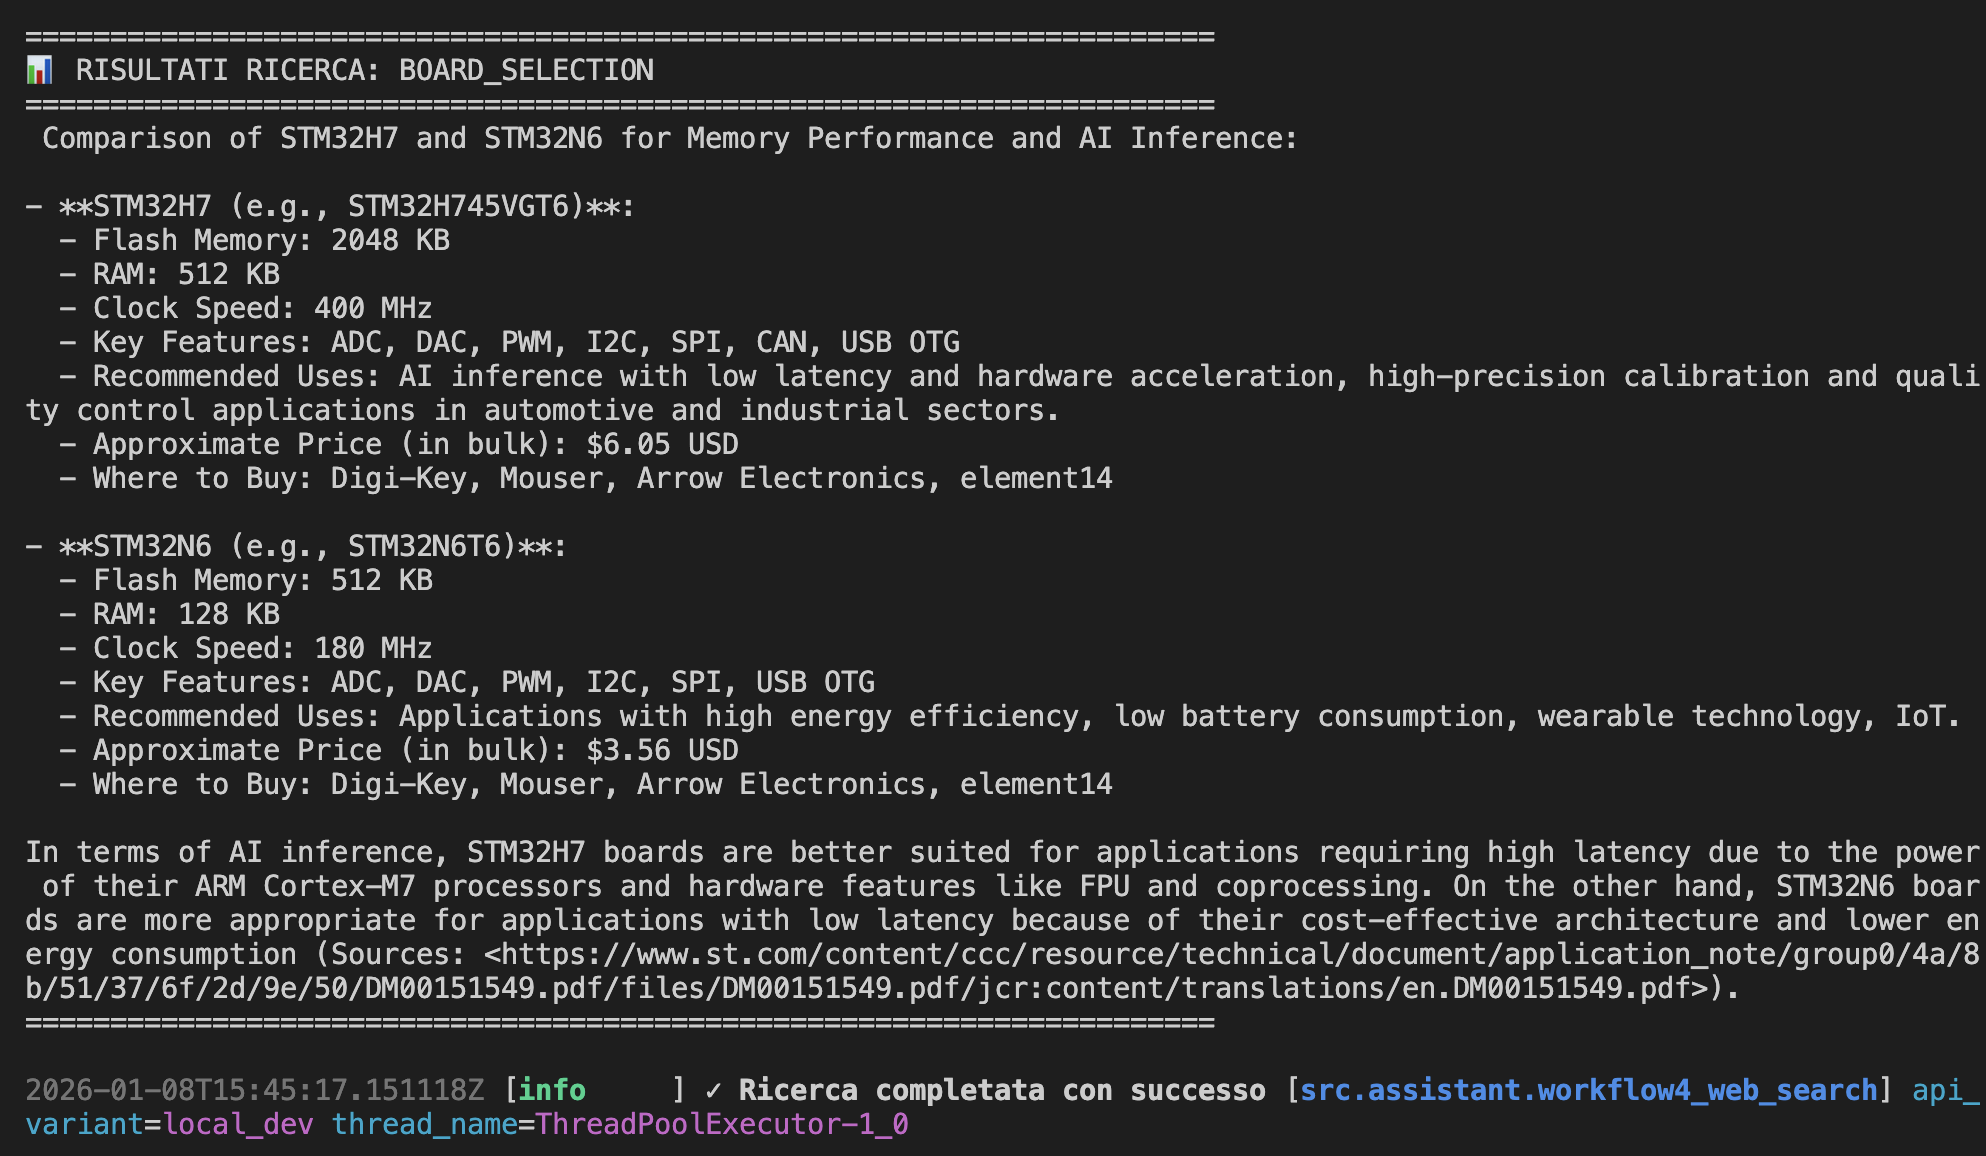
\includegraphics[width=0.9\textwidth]{chap4/figures/Screenshot 2026-01-08 at 16.46.34.png}
  \caption{Web Search Agent output for PyTorch-to-ONNX conversion query, demonstrating perfect Faithfulness (1.00) by strictly adhering to retrieved technical guides.}
  \label{fig:pytorch-onnx}
\end{figure}

\textbf{Test 4 -- Theoretical Comparison}: \textit{``TinyML vs Edge AI: differenze principali''}
\textbf{Best overall scores} (Answer Relevancy: 0.88, Contextual Relevancy: 0.86). The query's conceptual nature (definitions, comparisons) aligned well with academic sources (datasheets, whitepapers). High Contextual Relevancy confirms Google retrieved authoritative STMicroelectronics documentation. Output shown in Figure~\ref{fig:tinyml-edgeai}.

\begin{figure}[ht]
  \centering
  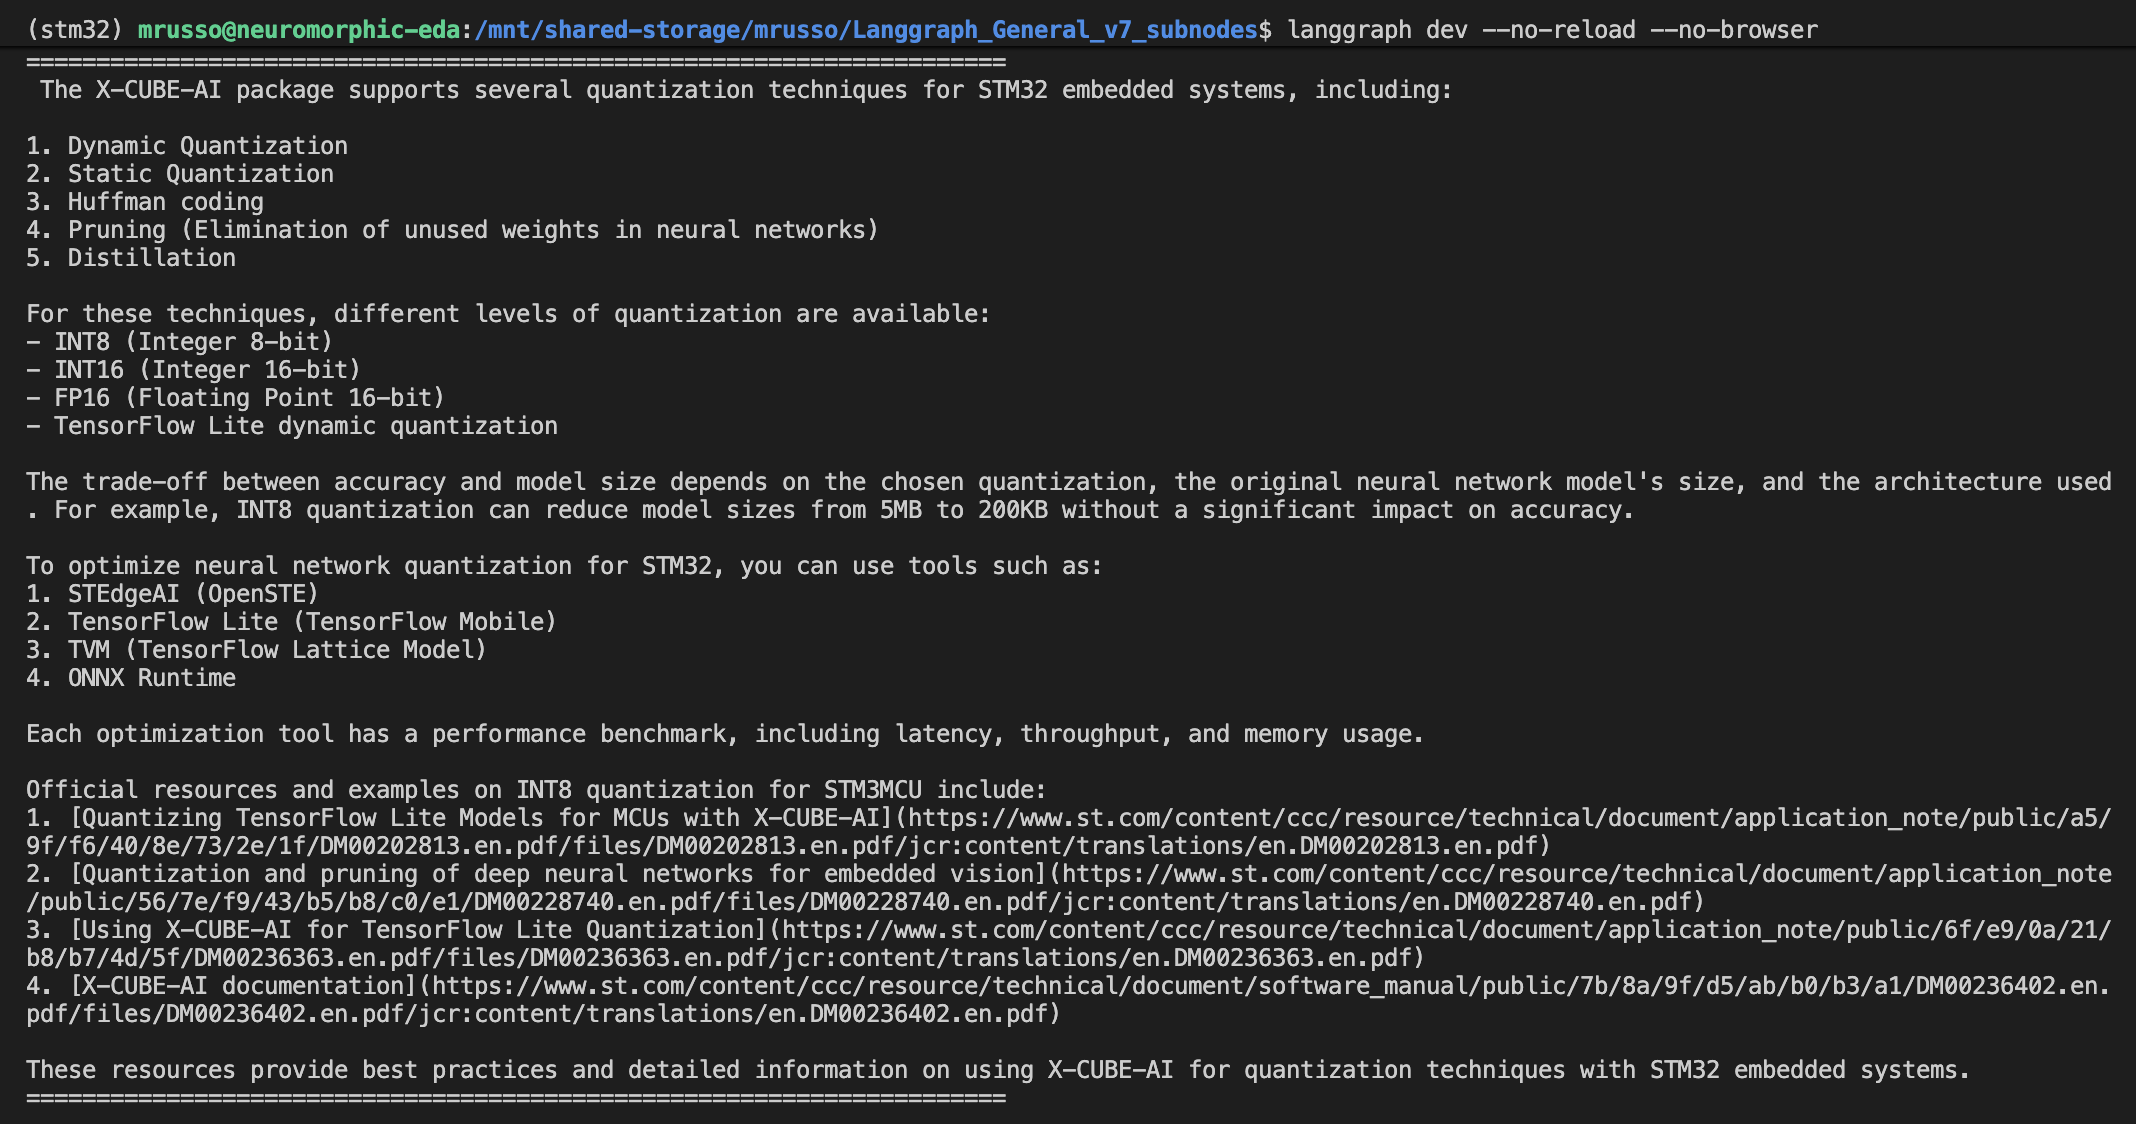
\includegraphics[width=0.9\textwidth]{chap4/figures/Screenshot 2026-01-08 at 16.50.55.png}
  \caption{Comparative analysis of TinyML vs. Edge AI paradigms, achieving highest Answer Relevancy (0.88) through precise conceptual distinction.}
  \label{fig:tinyml-edgeai}
\end{figure}

\textbf{Test 5 -- Hardware Comparison}: \textit{``Confronta STM32H7 e STM32N6 per performance AI''}
The \textbf{lowest Faithfulness (0.44)} reveals an interesting trade-off: the summary included precise part numbers (STM32H745VGT6, STM32N6T6) and bulk pricing (\$6.05, \$3.56) that were \textbf{not} present in the retrieved snippets. DeepEval correctly flagged this as potential hallucination (0.33). While useful for users, it demonstrates the LLM's reliance on pre-trained knowledge when retrieval is incomplete.

\subsection{Discussion}

\subsubsection{Aggregate Performance}
The system achieved consistent and revealing performance across all evaluated metrics. The consistently high scores for Contextual Relevancy (mean: 0.75, $\sigma$: 0.16; range: 0.56--0.90) firmly confirm the fundamental effectiveness of combining Google Search with targeted paragraph-level chunking. 

However, the wide variance observed in Faithfulness (mean: 0.71, $\sigma$: 0.22) starkly reflects a Faithfulness-Utility trade-off: highly procedural queries achieve perfect scores by strictly adhering to retrieved sources, whereas exploratory consulting queries exhibit lower scores due to helpful but ungrounded LLM enrichment. Reassuringly, the low average for Hallucination (mean: 0.14, $\sigma$: 0.14) confirms minimal outright fabrication, with the few non-zero scores accurately detecting highly specific claims, such as hardware pricing or exact part numbers, that were genuinely absent from the raw retrieval context.

\subsubsection{Faithfulness-Utility Trade-off}
A key finding of this evaluation is the distinctly inverse relationship observed between absolute Faithfulness and practical user utility. High Faithfulness (between 0.80 and 1.00) is invariably achieved when the LLM strictly paraphrases the retrieved documents, making it ideal for rigid technical procedures and precise academic definitions. However, low Faithfulness (between 0.44 and 0.60) frequently occurs when the LLM intelligently supplements the basic retrieval with its own pre-trained domain knowledge, such as adding standard pricing estimates or typical hardware specifications. While technically unfaithful to the search results, this enrichment produces significantly more useful answers for exploratory queries, albeit requiring slightly more cautious interpretation from the user.

This trade-off suggests the need for \textbf{context-aware metric weighting}: procedural queries should prioritize Faithfulness, while exploratory queries may tolerate lower Faithfulness in exchange for detailed answers.

\subsubsection{Threats to Validity}
Several threats to validity clearly apply to this rigorous evaluation. Concerning internal validity, the selected LLM temperature of 0.2 deliberately trades creative fluency for deterministic consistency; utilizing even lower values might marginally improve mathematical Faithfulness at the heavy cost of readability. 

Regarding external validity, the test cases were strictly limited to the STM32 and Edge AI domains, meaning successful generalization to wildly different embedded ecosystems like ESP32 or Arduino remains formally unverified. 

Finally, regarding construct validity, it is clear that the strict DeepEval Faithfulness metric aggressively penalizes helpful LLM enrichment, meaning that human domain experts might actually prefer ``unfaithful'' enriched answers despite their lower automated scores.

\subsection{Conclusion}
The experimental validation demonstrates that the Web Search Agent, augmented with DeepEval metrics, provides a \textbf{transparent, quantifiable quality assessment} of AI-generated technical guidance. The system achieves:
\begin{enumerate}
  \item High retrieval quality (avg. Contextual Relevancy: 0.75)
  \item Minimal hallucination (avg. Hallucination: 0.14)
  \item Adaptive behavior across query types (perfect Faithfulness for procedures, enriched answers for exploration)
\end{enumerate}

Future work should explore adaptive metric weighting, hybrid retrieval strategies (vector DB + web search), and user feedback integration to calibrate acceptable Faithfulness-Utility trade-offs for different stakeholder profiles (novice developers vs. domain experts).
